\providecommand{\Bezier}{B\'{e}zier}
\providecommand{\bezier}{b\'{e}zier}

\title{Calculus II Applications to \Bezier\ Curves: Normal, Tangent, and Bounds}
\author{Jeff W McGlynn}
\date{\today}

\documentclass[oneside]{article}
\usepackage{color} %used for font color
\usepackage{amssymb} %maths
\usepackage{amsmath} %maths
\usepackage[utf8]{inputenc} %useful to type directly diacritic characters
\usepackage{graphicx}
\usepackage{subfigure}

% Set up margins.
\usepackage[margin=1in]{geometry}

\begin{document}
\maketitle
\tableofcontents
\setcounter{tocdepth}{2}

\newpage

\section{Derivative}
\label{Derivative}

\subsection{General Equation}
The general equation for a \Bezier\ curve is:

\begin{equation}\label{bezier_general}
	\mathbf{B}(t) = \sum_{i=0}^n {n\choose i} (1 - t)^{n - i} t^i \mathbf{P}_i
\end{equation}

Since we are taking the derivative with respect to $t$, only the Bernstein polynomial effects the derivative.  The Bernstein polynomial is:

\[ B_{n,i}(t) = {n\choose i} (1 - t)^{n - i} t^i \]

Or, expanded:

\[ B_{n,i}(t) = \cfrac{n!}{i! (n - i)!} (1 - t)^{n - i} t^i \]

\subsection{Finding the Bernstein Polynomial's Derivative}

The derivative of this is:

\[ B_{n,i}'(t) = \cfrac{n!}{i! (n - i)!} [ it^{i - 1} (1 - t)^{n - i}] - \cfrac{n!}{i! (n - i)!}[t^i (n - i)(1 - t)^{n - i - 1}] \]

By simplifying and pulling out an $n$, this simplifies to:

\[ B_{n,i}'(t) = n \cfrac{(n - 1)!}{(i - 1)! (n - i)!} [ t^{i - 1} (1 - t)^{n - i}] - n \cfrac{(n - 1)!}{i! (n - i - 1)!}[t^i (1 - t)^{n - i - 1}] \]

Observe that this equation is now composed of two different Bernstein polynomials.  After substituting them in, the equation becomes:

\[ B_{n,i}'(t) = n [ B_{n-1,i-1}(t) - B_{n-1,i}(t) ] \]

The derivative of the internal Bernstein polynomial is now known.  It is substituted back into the general equation for a \Bezier\ curve:

\[ \mathbf{B}'(t) = \sum_{i=1}^{n} B_{n,i}'(t) \mathbf{P}_i \]

\[ \mathbf{B}'(t) = \sum_{i=1}^{n} n [ B_{n-1,i-1}(t) - B_{n-1,i}(t) ] \mathbf{P}_i \]

\begin{equation}\label{bezier_der_close}
	\mathbf{B}'(t) = \sum_{i=0}^{n-1} n [ B_{n-1,i}(t) - B_{n-1,i+1}(t) ] \mathbf{P}_{i+1}
\end{equation}

Note the interference pattern that is created by created by subtracting $B_{n,i+1}$ in \eqref{bezier_der_close}.  Using this, the derivative of \eqref{bezier_general} can be rewritten as:

\subsection{General Derivative}

\begin{equation}\label{bezier_deriv}
	\mathbf{B}'(t) = \sum_{i=0}^{n-1} n B_{n-1,i}(t) [ \mathbf{P}_{i+1} - \mathbf{P}_i ]
\end{equation}

This is the general derivative of a \Bezier\ curve.

\section{Normal Vector}

\begin{figure}[htp]
\begin{center}
	
	\subfigure[Cubic \Bezier\ Curve]{
		\label{fig:bezier_spline}
		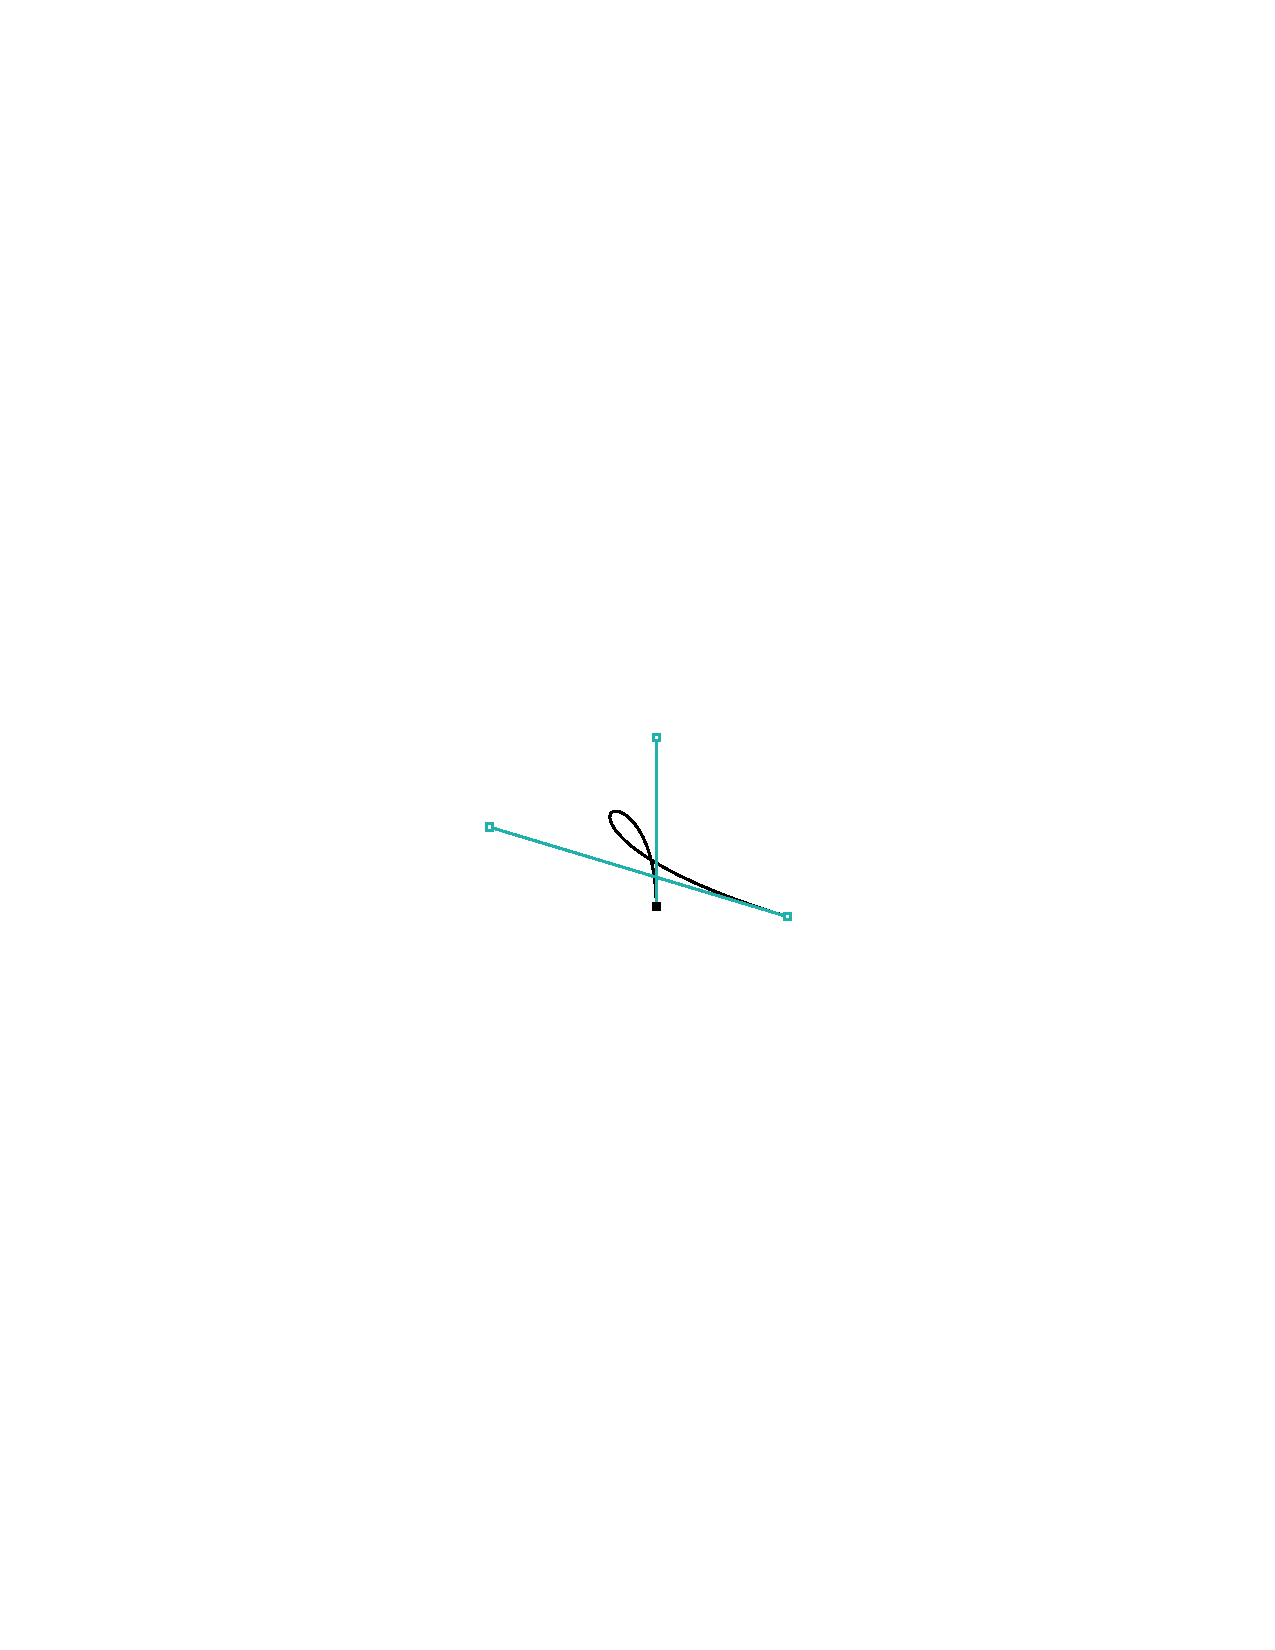
\includegraphics{figure_bezier_spline}
	}
	\subfigure[Derivative of \ref{fig:bezier_spline}]{
		\label{fig:bezier_spline_deriv}
		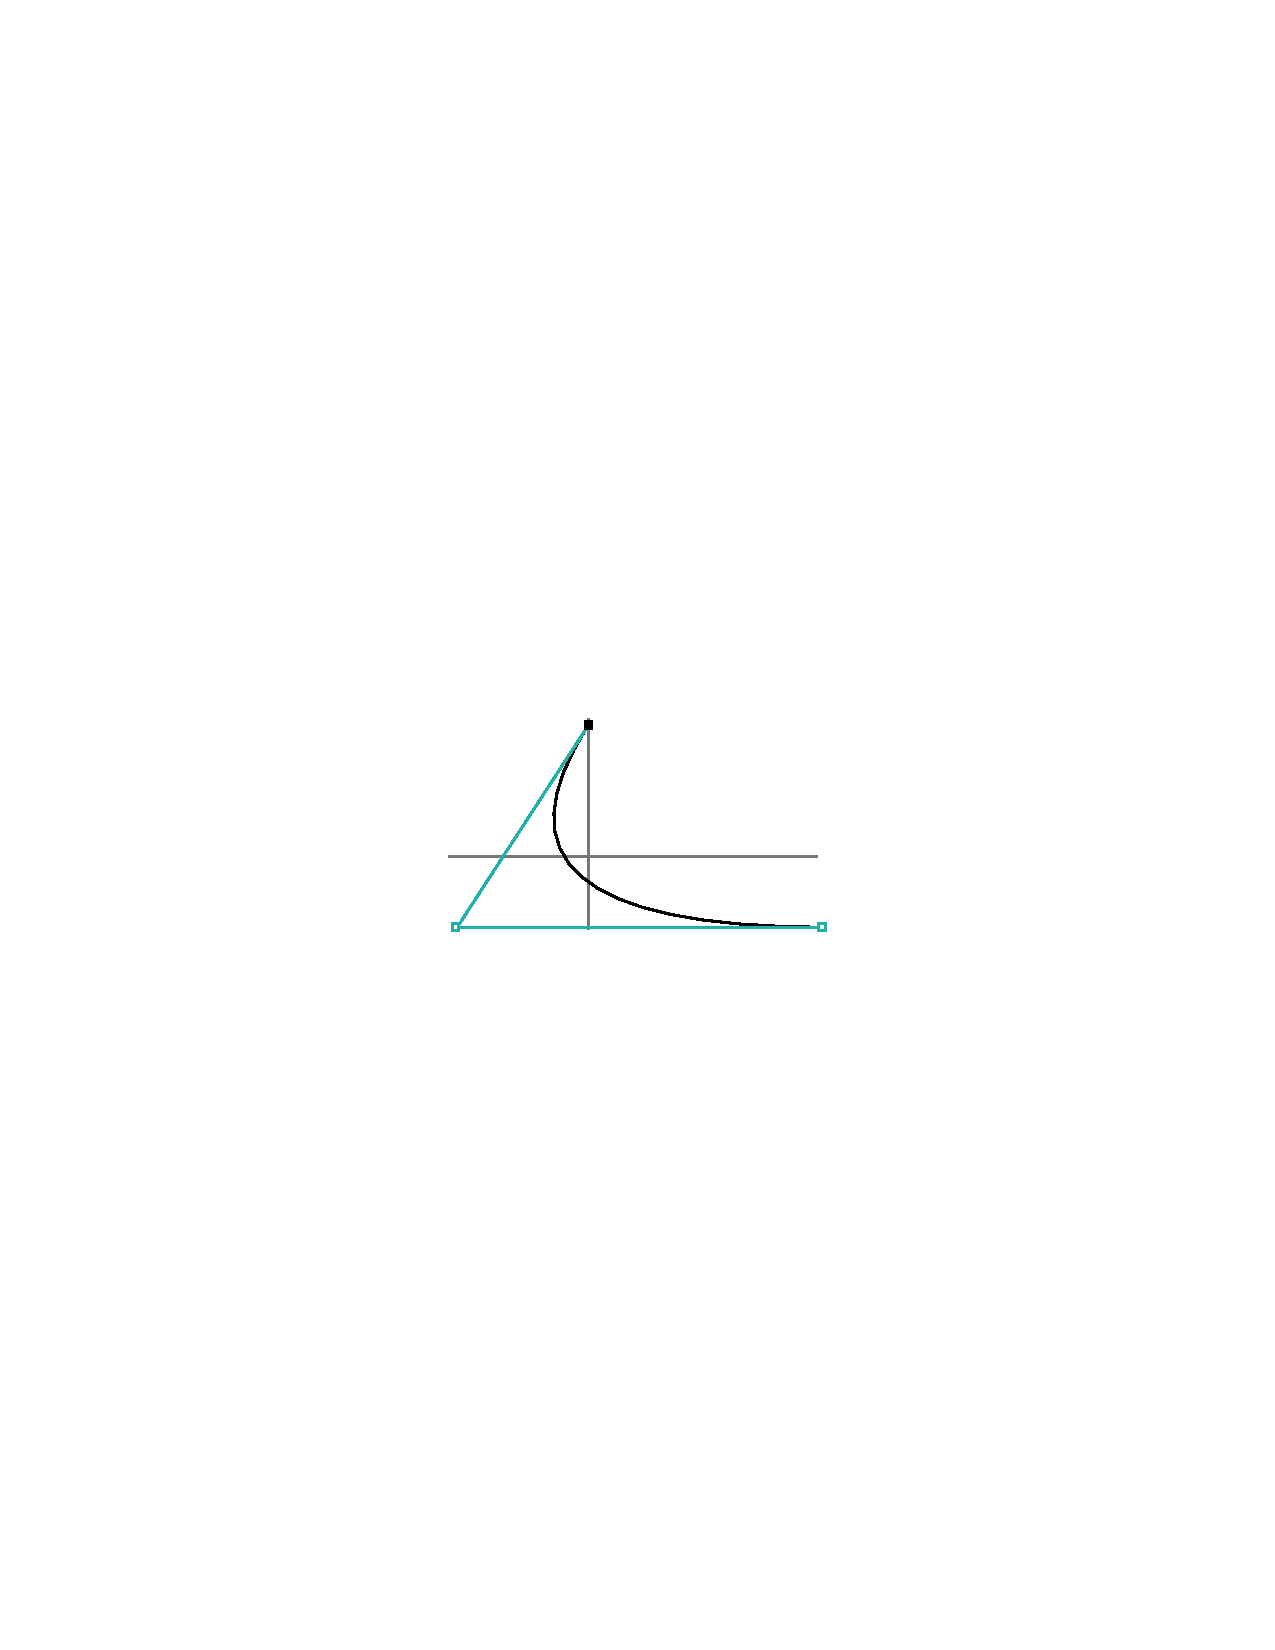
\includegraphics{figure_bezier_spline_deriv}
	}
	
	\caption{Cubic \Bezier\ Curve and Derivative}
\end{center}
\end{figure}

TODO.

\end{document}
